\let\negmedspace\undefined
\let\negthickspace\undefined
\documentclass[journal]{IEEEtran}
\usepackage[a5paper, margin=10mm, onecolumn]{geometry}
%\usepackage{lmodern} % Ensure lmodern is loaded for pdflatex
\usepackage{tfrupee} % Include tfrupee package

\setlength{\headheight}{1cm} % Set the height of the header box
\setlength{\headsep}{0mm}     % Set the distance between the header box and the top of the text

\usepackage{gvv-book}
\usepackage{gvv}
\usepackage{cite}
\usepackage{amsmath,amssymb,amsfonts,amsthm}
\usepackage{algorithmic}
\usepackage{graphicx}
\usepackage{textcomp}
\usepackage{xcolor}
\usepackage{txfonts}
\usepackage{listings}
\usepackage{enumitem}
\usepackage{mathtools}
\usepackage{gensymb}
\usepackage{comment}
\usepackage[breaklinks=true]{hyperref}
\usepackage{tkz-euclide} 
\usepackage{listings}
% \usepackage{gvv}                                        
\def\inputGnumericTable{}                                 
\usepackage[latin1]{inputenc}                                
\usepackage{color}                                            
\usepackage{array}                                            
\usepackage{longtable}                                       
\usepackage{calc}                                             
\usepackage{multirow}                                         
\usepackage{hhline}                                           
\usepackage{ifthen}                                           
\usepackage{lscape}
\begin{document}

\bibliographystyle{IEEEtran}
\vspace{3cm}

\title{CHAPTER - 6\\Application of Derivatives}
\author{EE24BTECH11061 - Rohith Sai}
% \maketitle
% \newpage
% \bigskip
{\let\newpage\relax\maketitle}

\renewcommand{\thefigure}{\theenumi}
\renewcommand{\thetable}{\theenumi}
\setlength{\intextsep}{10pt} % Space between text and floats

\numberwithin{figure}{enumi}
\renewcommand{\thetable}{\theenumi}

\section*{Exercise : 6.5}
\begin{enumerate}
\item [5.2)] Find the absolute maximum value and the absolute minimum value of the function $f\brak{x} = \sin{x} + \cos{x} \,, x \in \sbrak{0, \pi}$\\
\textbf{Theoretical Solution:}\\
Given the function:
\begin{align}
    f(x) = \sin x + \cos x, \text{ where } x \in [0, \pi]
\end{align}

To find the critical points, we differentiate $f(x)$ with respect to $x$:
\begin{align}
    \frac{df}{dx} = \cos x - \sin x
\end{align}

Setting the derivative equal to zero:
\begin{align}
    \cos x - \sin x = 0 \\
    \cos x = \sin x
\end{align}

This occurs when:
\begin{align}
    x = \frac{\pi}{4}
\end{align}

Now, let's evaluate $f(x)$ at the critical point and the boundaries of the interval:

\begin{itemize}
    \item At $x = 0$:
    \begin{align}
        f(0) = \sin(0) + \cos(0) = 0 + 1 = 1
    \end{align}
    
    \item At $x = \frac{\pi}{4}$:
    \begin{align}
        f\left(\frac{\pi}{4}\right) = \sin\left(\frac{\pi}{4}\right) + \cos\left(\frac{\pi}{4}\right) = \frac{\sqrt{2}}{2} + \frac{\sqrt{2}}{2} = \sqrt{2}
    \end{align}
    
    \item At $x = \pi$:
    \begin{align}
        f(\pi) = \sin(\pi) + \cos(\pi) = 0 - 1 = -1
    \end{align}
\end{itemize}

Therefore, the maximum value of $f(x)$ in the interval $[0, \pi]$ is $\sqrt{2}$, and the minimum value is $-1$.\\

\textbf{Computational Solution (Solved):}\\

To find the maximum and minimum values of the function $f(x) = \sin x + \cos x$ on the interval $x \in [0, \pi]$, we use iterative methods like gradient ascent and gradient descent.

\vspace{2mm}

The gradient ascent method is used to find the maximum value of a function by following the direction of the positive gradient. The iterative formula for gradient ascent is given by:
\begin{align}
    x_{n+1} = x_n + \eta \cdot \frac{df}{dx}
\end{align}
where $x_n$ is the current value of $x$, $x_{n+1}$ is the next value of $x$, $\eta$ is the learning rate (a small positive number), and $\frac{df}{dx}$ is the derivative of the function at $x_n$.

First, we compute the derivative of $f(x)$:
\begin{align}
    \frac{df}{dx} = \cos x - \sin x
\end{align}

To apply gradient ascent, choose an initial point $x_0$ within the interval $[0, \pi]$, and apply the gradient ascent formula iteratively until convergence. The iteration stops when the gradient becomes zero. We find the maximum at $x = \frac{\pi}{4}$ because the gradient changes sign around this point.

The function value at $x = \frac{\pi}{4}$ is:
\begin{align}
    f\left(\frac{\pi}{4}\right) = \sin\left(\frac{\pi}{4}\right) + \cos\left(\frac{\pi}{4}\right) = \sqrt{2}
\end{align}
Therefore, the absolute maximum value of $f(x)$ is $\sqrt{2}$ at $x = \frac{\pi}{4}$.

\vspace{2mm}

The gradient descent method is used to find the minimum value of a function by following the direction of the negative gradient. The iterative formula for gradient descent is given by:
\begin{align}
    x_{n+1} = x_n - \eta \cdot \frac{df}{dx}
\end{align}

Starting with an initial point $x_0$ within the interval $[0, \pi]$, we apply the gradient descent formula iteratively until convergence. The iteration stops when the gradient becomes zero. We find the minimum at $x = \pi$ because the gradient changes sign around this point.

The function value at $x = \pi$ is:
\begin{align}
    f(\pi) = \sin(\pi) + \cos(\pi) = -1
\end{align}
Therefore, the absolute minimum value of $f(x)$ is $-1$ at $x = \pi$.

\vspace{2mm}

The computational results are summarized as follows:
\begin{align}
    \text{Absolute Maximum:} \quad f(x) = \sqrt{2} \text{ at } x = \frac{\pi}{4} \\
    \text{Absolute Minimum:} \quad f(x) = -1 \text{ at } x = \pi
\end{align}
The graph of the function $f(x) = \sin{x} + \cos{x}$ representing the maximum and minimum values is shown below:
\begin{figure}
    \centering
    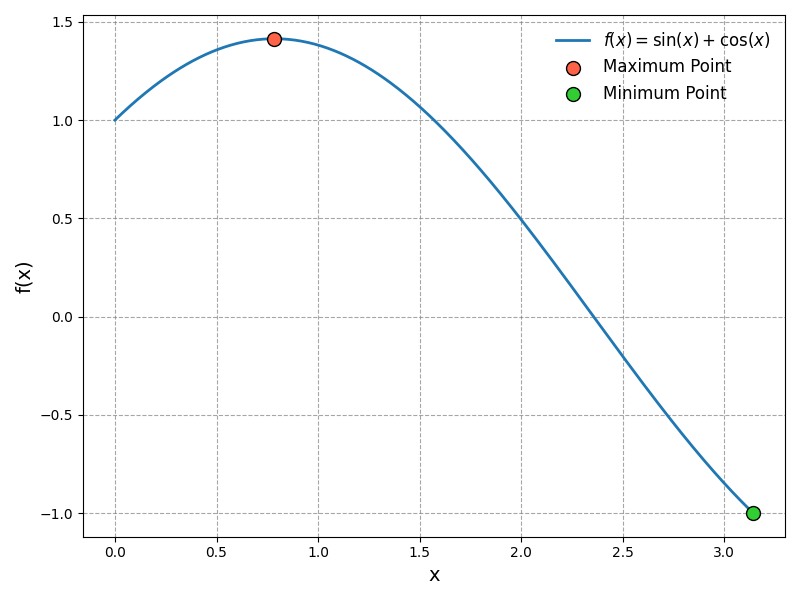
\includegraphics[width=\columnwidth]{figs/fig.png}
\end{figure}
\end{enumerate}
\end{document}